\documentclass{article}
\usepackage{tikz}
\usepackage{graphicx} % Required for inserting images

\title{Implementare automat finit}
\author{Alexandru Scanteie}
\maketitle
\begin{document}

\begin{center}
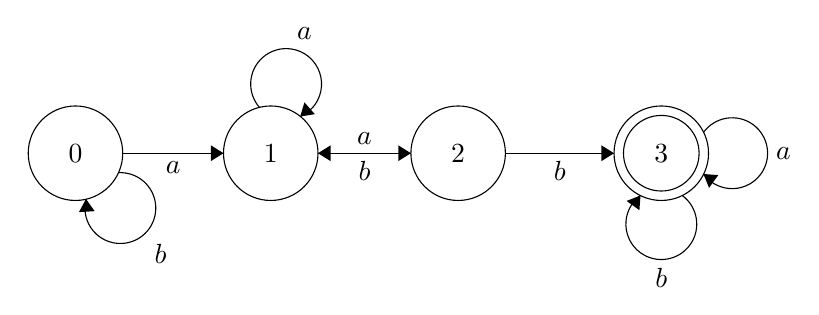
\begin{tikzpicture}[scale=0.2]
\tikzstyle{every node}+=[inner sep=0pt]
\draw [black] (20.8,-36.1) circle (3);
\draw (20.8,-36.1) node {$0$};
\draw [black] (33.2,-36.1) circle (3);
\draw (33.2,-36.1) node {$1$};
\draw [black] (45.1,-36.1) circle (3);
\draw (45.1,-36.1) node {$2$};
\draw [black] (58,-36.1) circle (3);
\draw (58,-36.1) node {$3$};
\draw [black] (58,-36.1) circle (2.4);
\draw [black] (23.8,-36.1) -- (30.2,-36.1);
\fill [black] (30.2,-36.1) -- (29.4,-35.6) -- (29.4,-36.6);
\draw (27,-36.6) node [below] {$a$};
\draw [black] (23.52,-37.337) arc (93.28941:-194.71059:2.25);
\draw (26.2,-41.82) node [below] {$b$};
\fill [black] (21.47,-39.01) -- (21.02,-39.84) -- (22.02,-39.78);
\draw [black] (32.49,-33.197) arc (221.47119:-66.52881:2.25);
\draw (35.34,-28.92) node [above] {$a$};
\fill [black] (35.07,-33.77) -- (36,-33.62) -- (35.34,-32.87);
\draw [black] (36.2,-36.1) -- (42.1,-36.1);
\fill [black] (42.1,-36.1) -- (41.3,-35.6) -- (41.3,-36.6);
\draw (39.15,-36.6) node [below] {$b$};
\draw [black] (42.1,-36.1) -- (36.2,-36.1);
\fill [black] (36.2,-36.1) -- (37,-36.6) -- (37,-35.6);
\draw (39.15,-35.6) node [above] {$a$};
\draw [black] (48.1,-36.1) -- (55,-36.1);
\fill [black] (55,-36.1) -- (54.2,-35.6) -- (54.2,-36.6);
\draw (51.55,-36.6) node [below] {$b$};
\draw [black] (60.68,-34.777) arc (144:-144:2.25);
\draw (65.25,-36.1) node [right] {$a$};
\fill [black] (60.68,-37.42) -- (61.03,-38.3) -- (61.62,-37.49);
\draw [black] (59.323,-38.78) arc (54:-234:2.25);
\draw (58,-43.35) node [below] {$b$};
\fill [black] (56.68,-38.78) -- (55.8,-39.13) -- (56.61,-39.72);
\end{tikzpicture}
\end{center}

\section*{Implementarea unui automat finit}

\begin{verbatim}
Q = {0, 1, 2, 3}
Sigma = {'a', 'b'}
Delta = {
    (0, 'a'): 1,
    (0, 'b'): 0,
    (1, 'a'): 1,
    (1, 'b'): 2,
    (2, 'a'): 1,
    (2, 'b'): 3,
    (3, 'a'): 3,
    (3, 'b'): 3
}
q0 = 0
F = {3}

def accepta_cuvant(w):
q = q0
for lit in w:
    q = Delta.get((q, lit), None)
    if q is None:
        return False
    return q in F

w = 'ababab'
print(accepta_cuvant(w)) # False
w = 'abb'
print(accepta_cuvant(w)) # True
\end{verbatim}

\end{document}